\documentclass[10pt,fullscreen=true, bookmarks=false]{beamer}
\usepackage{fancyhdr}
%\usepackage{lipsum}
%\usepackage{marvosym}
\usepackage{amssymb}
\usepackage{bbm}
\usepackage{ucs}
\usepackage[utf8x]{inputenc}
%\usepackage[english,russian]{babel}
\usepackage[T2A]{fontenc}
%\usepackage[T1]{fontenc}
%\usepackage{textcomp}
%\usepackage{amsmath}
%\usepackage{amsfonts}
%\usepackage{amssymb}
\usepackage{listings}
\usepackage{graphicx}
\usepackage{blindtext}
\usepackage{enumitem}

%\usepackage[utf8x]{inputenc}
%\usepackage[utf8]{inputenc}
%\usepackage[T2A]{fontenc}
%\usepackage[english,russian]{beamer}
\usepackage{xcolor}
\usepackage{hyperref}
\usepackage{listings}


\usetheme{default}
\title{Lab 1. Part II. Lexer for cool. C++ and GNU. }

\author{I.~Gorban}

\date{Mipt (Ilab), 10.09.2018}

\begin{document}

% 1-st page
\begin{frame}
\titlepage
\end{frame}

% 3-d page
\begin{frame}[fragile]
\frametitle{Что вы здесь не увидите}

1. Здесь не будет рассмотрен хороший стиль С++ (для этого смотрите - лекции Константина Владимирова.

2. Сегодня не будет рассмотренна внутренняя архитектура компилятора cool (будет позже).

3. Полный справочник по С++ - настоятельно рекомендован к изучению (и дополнению) \url{https://cppreference.com/} - есть русская версия.

4. Точных и формальных определений. Здесь будут даны определения "as is". Для того, чтобы дать хотя бы примерное представление о предмете разговора.

5. Ссылки с описанием 

\url{https://s3-us-west-1.amazonaws.com/prod-edx/Compilers/ProgrammingAssignments/PA1.pdf}

\url{https://lagunita.stanford.edu/c4x/Engineering/Compilers/asset/cool_manual.pdf}

\url{https://lagunita.stanford.edu/c4x/Engineering/Compilers/asset/cool-tour.pdf}

\AtBeginEnvironment{tabular}{\tiny}
\tableofcontents[pausesections]
\end{frame}

\begin{frame}[fragile]
\frametitle{Flex}

\begin{figure}
  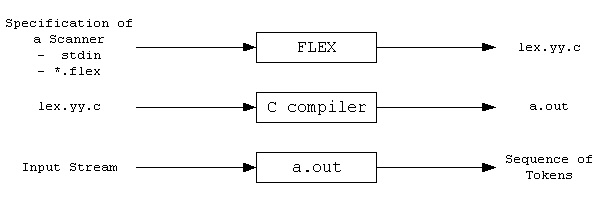
\includegraphics[width=\linewidth]{flex.jpg}
  \caption{Последовательность работы flex.}
\end{figure}

Здесь {\bf Flex} - программа для генерации лексических анализаторов, обычно используемая совместно с генератором синтаксических анализаторов. {\bf C compiler} - gcc.

\tableofcontents[pausesections]
\end{frame}


\begin{frame}[fragile]
\frametitle{COOL grammar}

Грамматика COOL :
\begin{lstlisting}[basicstyle=\tiny]
program ::= [[class; ]]+
  class ::= class TYPE [inherits TYPE] { [[feature; ]]}
feature ::= ID( [ formal [[, formal]] ] ) : TYPE { expr }
          | ID : TYPE [ <- expr ]
 formal ::= ID : TYPE
   expr ::= ID <- expr
          | expr[@TYPE].ID( [ expr [[, expr]] ] )
          | ID( [ expr [[, expr]] ] )
          | if expr then expr else expr fi
          | while expr loop expr pool
          | { [[expr; ]]+}
          | let ID : TYPE [ <- expr ] [[, ID : TYPE [ <- expr ]]] in expr
          | case expr of [[ID : TYPE => expr; ]]+esac
          | new TYPE
          | isvoid expr
          | expr (+|-|*|/) expr
          | ~expr
          | expr < expr
          | expr <= expr
          | expr = expr
          | not expr
          | (expr)
          | ID
          | integer
          | string
          | true
          | false
\end{lstlisting}

\tableofcontents[pausesections]
\end{frame}




\begin{frame}[fragile]
\frametitle{COOL lex example in work}

Давайте рассмотрим лексемы "TYPEID", "OBJECTID", "INT\_CONST" и "STR\_CONST".

TYPEID - имя типа, такое как String, Int, Foo, Bar (по соглашению типами считаются все слова, начинающиеся с заглавной буквы).

OBJECTID - имя обьекта, например str, myint, i (по соглашению именами обьекта считаются все слова, начинающиеся с прописной буквы)

INT\_CONST - константное значение числа.

STR\_CONST - константное значение строки.

Чтобы сохранить информацию об имени типа - (например не хочется хранить 10 раз одно и то же имя), связка программ flex-bison работает через cool\_yylval. Symbol - хранит указатель на элемент в таблице символов.

\begin{lstlisting}[language=C++,breaklines]
yylval.symbol = stringtable.add_string(yytext);
\end{lstlisting}


Теперь разберемся с исходным кодом.

\tableofcontents[pausesections]
\end{frame}

\begin{frame}[fragile]
\frametitle{Cool flex}

Вот так выглядит реализация самого простого cool-компилятора:
\begin{lstlisting}[language=bash]
$ cat mycoolc
#!/bin/csh -f
./lexer $* | ./parser $* | ./semant $* | ./cgen $*
\end{lstlisting}

То есть результат лексера - подается на вход парсеру, результат парсера на вход семантическому анализатору. Результат семантического анализатора на вход кодогенератора.


Пример токенов и лексем:

\begin{tabular}{|l|l|l|}
\hline
тип токена & примеры лексем &	описание \\
\hline
num 	& 257 &	число \\
\hline
id &	 Ident951 &	идентификатор \\
\hline
relop &	<= & 	операция отношения \\
\hline
string & 	«Cимвол» &	строчная постоянная \\
\hline
\end{tabular}


\tableofcontents[pausesections]
\end{frame}




\begin{frame}[fragile]
\frametitle{Шаблоны внутри COOL}

Класс list находится в include/list.h. Класс StringTable 

\begin{lstlisting}[language=C++,breaklines]
template <class T>
class List {
private:
  T *head;
  List<T>* tail;
public:
  List(T *h,List<T>* t = NULL): head(h), tail(t){ }

  T *hd() const       { return head; }
  List<T>* tl() const { return tail; }
};

template <class Elem>
class StringTable
{
protected:
   List<Elem> *tbl;   // a string table is a list
   int index;         // the current index

\end{lstlisting}


\tableofcontents[pausesections]
\end{frame}



% 3
\begin{frame}[fragile]
\frametitle{C++ Классы определения}

{\bfКласс} - это тип, определяемый пользователем, для которого определен ряд методов.

{\bfМетоды класса} - функции, описанные внутри тела класса.

{\bfОбьект класса} - элемент, имеющий размер равный размеру класса, из которого можно вызывать методы класса.

Описание класса, это не точное определение, сюда можно навесить еще минимум 4 аттрибута ( "-" играет роль определителя регекспа):
\begin{lstlisting}[language=C++,breaklines]
class class_name (- : ancestor_list -)-?
{
   (- (- public: | private: | protected: -)-?
	  (- virtual -)? (- static -)? type Method_name((- variables -)-*) (- definition | ; -)
	  (- static -)-?  type variable_name (declaration)? ;
   -)*
} 
\end{lstlisting}


\tableofcontents[pausesections]
\end{frame}


\begin{frame}[fragile]
\frametitle{C++ Конструктор, деструктор, статические члены и методы.}

{\bfКонструктор} - метод, который имеет название, совпадающее с именем класса, ничего не возвращает и логически выполняет роль инициализации обьекта. Может принимать аргументы. В случае, если аргумент - константный обьект того же класса - называется конструктором копирования

{\bfДеструктор} - метод, противоположный конструктору, то есть логически выполняет роль очистки. Так же ничего не возвращает. Название соотвествует "\textasciitilde имя\_класса", не имеет аргументов.

{\bfСтатические члены и аттрибуты} - это члены и аттрибуты, которые не привязанны к какому-либо обьекту, однако логически должны использоваться только в связке с ними (или совсем без конструирования).

\tableofcontents[pausesections]
\end{frame}


\begin{frame}[fragile]
\frametitle{C++ Виртуальные методы, таблица виртуальных функций, перегрузка операторов}

{\bfВиртуальный метод} - метод обьекта, имеющий смысл только в цепочке наследования. Такой метод будет вызываться у обьекта вне зависимости, какой указатель используется.
\newline 

\begin{tabular}{|l|l|l|}
\hline
Offset	& Method name(A) & Method name(B : public A)\\
\hline
0x0000	& void A::foo() & void A::foo()\\
\hline
0x0004 	& virtual void foo(int) & virtual void foo(int) \\
\hline
0x0008 	& void foo(bool) &  void foo(char)\\
\hline
\end{tabular}

(В таблице указанны отступы относительно начала таблицы для для каждого класса)

{\bfПерегрузка операторов} - механизм, с помощью которого можно определить поведение обьектов класса при использование операторов "+","-","()","[]" и т.д. 

\tableofcontents[pausesections]
\end{frame}


\begin{frame}[fragile]
\frametitle{C++ Шаблонные функции, шаблонные классы, инстанциация}

{\bfШаблонная функция} - функция, некоторые типы аргументов или аргументов заданы как шаблоны.

\begin{lstlisting}[language=C++,breaklines]
template<typename T>
void f(T s) { std::cout << s << '\n'; }
int main()
{
	// instantiation here 
    f<double>(1); f<>('a'); f(7); void (*ptr)(std::string) = f;
}
\end{lstlisting}


{\bfШаблонные классы} - полностью аналогичны функцям, только шаблонный параметр не ограничивается аргументами (то есть может использоваться шире).

{\bfИнстанциация} - точка в коде, где происходит конкретизация обьекта или где явно указанно, какими типами будет конкретизирован шаблон.

\tableofcontents[pausesections]
\end{frame}

\begin{frame}[fragile]
\frametitle{GCC}

\begin{figure}
  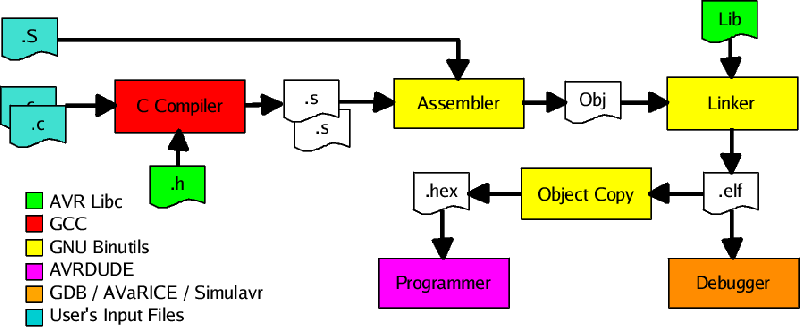
\includegraphics[width=\linewidth]{avrgcc-compilerchain.png}
  \caption{Фазы компиляции gcc без препроцессора.}
\end{figure}

\tableofcontents[pausesections]
\end{frame}

\begin{frame}[fragile]
\frametitle{GCC типы файлов}
\begin{itemize}
\item file.c  - Исходный код на C, который должен быть препроцессирован.
    \item file.i  - Исходный код на C, который не должен быть препроцессирован.
    \item file.s  - Код на языке ассемблера
    \item file.S / file.sx  - Код на языке ассемблера, который должен быть препроцессирован.
    \item file.cpp (cc / cp / cxx / CPP / c++ / C)   -  Исходный код на C++, который должен быть препроцессирован.
    \item file.h - Заголовочный файл для языков C, C++, Objective-C или Objective-C++ для добавления на этапе препроцессинга.
    \item file.hh (H / hp / hxx / hpp /HPP / h++ / tcc) - Заголовочные файлы на C++
\end{itemize}

\tableofcontents[pausesections]
\end{frame}


\begin{frame}[fragile]
\frametitle{GCC препроцессор, ассемблер}

Рассматриваемый пример:

\begin{lstlisting}[language=C++]
int f(int x)
{
	return 1 + x;
}
#define SQR(x) ((x)*(x))
unsigned sqr (int x) { return x*x; }
int main()
{
	int x = 8;
	unsigned t_slow = SQR(f(x));
	unsigned t_fast = sqr(f(x));
	return t_fast + t_slow;
}
\end{lstlisting}
\tableofcontents[pausesections]
\end{frame}


\begin{frame}[fragile]
\frametitle{GCC препроцессор, ассемблер}

Для получения результата препроцессора:
\begin{lstlisting}[language=bash]
gcc -E 01.cpp
\end{lstlisting}

Для получения ассемблерного файла :
\begin{lstlisting}[language=bash]
gcc 01.cpp -S -o 01.S
# Demangle
c++filt _Z3sqri
\end{lstlisting}

Для запуска ассемблера:
\begin{lstlisting}[language=bash]
as 01.S -o main.o
\end{lstlisting}

Для линковки (можно посмотреть опции вашего запуска, выполнив gcc 01.cpp -v ):

\begin{lstlisting}[breaklines]
ld -m elf_x86_64  -dynamic-linker /lib64/ld-linux-x86-64.so.2  /usr/lib/x86_64-linux-gnu/Scrt1.o /usr/lib/x86_64-linux-gnu/crti.o -L/usr/lib/gcc/x86_64-linux-gnu/8  main.o -lgcc  -lc /usr/lib/gcc/x86_64-linux-gnu/8/crtendS.o /usr/lib/x86_64-linux-gnu/crtn.o
\end{lstlisting}

\tableofcontents[pausesections]
\end{frame}


\begin{frame}[fragile]
\frametitle{GCC binutils отладочная информация}

Для чтения таблицы имён обьектного файла можно воспользоваться программой nm
\begin{lstlisting}[language=bash]
nm a.out
\end{lstlisting}

Для поиска печатных символов (строк, имен функций) можно воспользоваться программой strings
\begin{lstlisting}[language=bash]
strings a.out
\end{lstlisting}

Для получения информации о секциях, можно воспользоваться программой size
\begin{lstlisting}[language=bash]
size a.out
\end{lstlisting}

Примеры секций:
\begin{itemize}
    \item .text — содержит код программы
    \item .bss — неинициализированные переменные
    \item .data — инициализированные переменные
    \item .interp — путь к бинарному интерпретатору
    \item .init — выполняется до вызова точки входа
\end{itemize}

\tableofcontents[pausesections]
\end{frame}

\begin{frame}[fragile]
\frametitle{GCC binutils}

Для получения ассемблера из обьектного файла существует функция Objdump
\begin{lstlisting}[language=bash]
objdump -dx a.out > a.asm
\end{lstlisting}

Если необходимо узнать, какая строка соответвует 
\begin{lstlisting}[language=bash]
addr2line 0x1145 ./a.out
\end{lstlisting}

Для компиляции с дополнительными отладочными символами необходимо при компиляции подать опцию "-g" :
\begin{lstlisting}[language=bash]
gcc -g 01.cpp
\end{lstlisting}

Для запуска отладчика необходимо подать программу, скомпилированную с отладочными символами на gdb

\begin{lstlisting}[language=bash]
gdb ./a.out
# -> gdb information here
(gdb) help
# -> help information
(gdb) break main
Breakpoint 1 at 0x114d: file 01.cpp, line 13.
(gdb) run
Breakpoint 1, main () at 01.cpp:13
13		int x = 8;
\end{lstlisting}

\tableofcontents[pausesections]
\end{frame}


\begin{frame}[fragile]
\frametitle{Ссылки}

Грамматика C:
\url{https://www.lysator.liu.se/c/ANSI-C-grammar-l.html}
\url{https://www.lysator.liu.se/c/ANSI-C-grammar-y.html}

Грамматика C++

\url{http://www.nongnu.org/hcb/}

Грамматика Rust
\url{https://github.com/rust-lang/rust/tree/master/src/grammar}

Курс С++ от Смаля (СПБГУ)
\url{https://stepik.org/lesson/555/}

Список опций для отладки
\url{https://gcc.gnu.org/onlinedocs/gcc/Debugging-Options.html}


Лекции Константина Владимирова 
\url{https://sourceforge.net/projects/cpp-lects-rus/}

\tableofcontents[pausesections]
\end{frame}




\end{document}